\begin{figure*}
  \begin{subfigure}[b]{\textwidth}
    \centering
    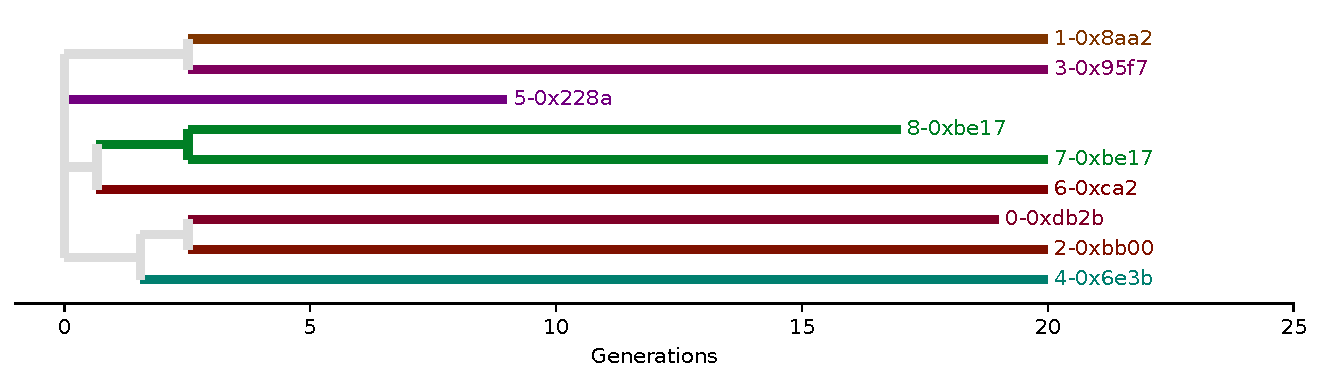
\includegraphics[width=\textwidth]{binder-wse-sketches/binder/teeplots/genome=hsurftiltedsticky_tagged+replicate=debd0010-f2aa-4679-aac6-b7ce94a2482a+viz=draw-biopython-tree+ext=}
    \caption{20 generations}
    \label{fig:tagged_other}
  \end{subfigure}

  \begin{subfigure}[b]{\textwidth}
    \centering
    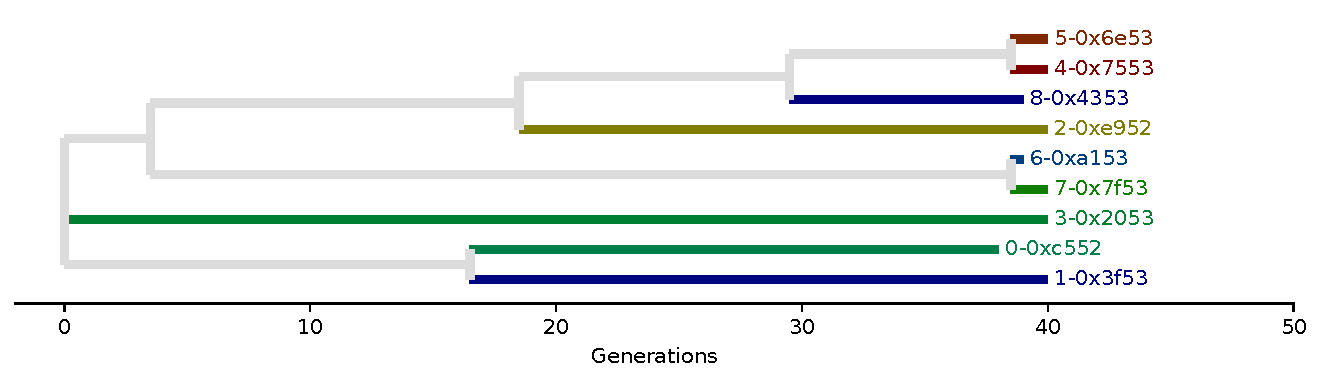
\includegraphics[width=\textwidth]{binder-wse-sketches/binder/teeplots/genome=hsurftiltedsticky_tagged+replicate=14302969-8474-4577-806b-4540da18c605+viz=draw-biopython-tree+ext=}
    \caption{40 generations}
    \label{fig:tagged_other}
  \end{subfigure}

  \begin{subfigure}[b]{\textwidth}
    \centering
    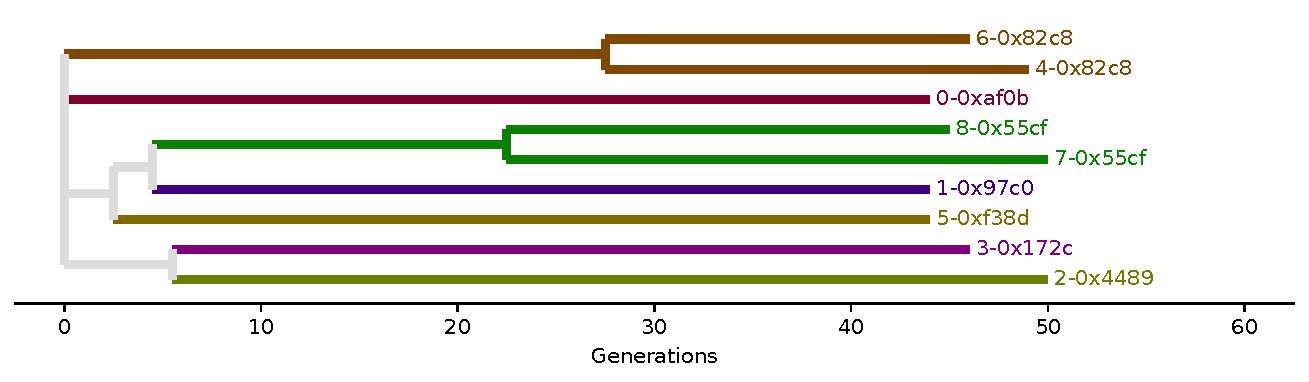
\includegraphics[width=\textwidth]{binder-wse-sketches/binder/teeplots/genome=hsurftiltedsticky_tagged+replicate=c830e722-ad66-48ed-a02f-2aa994dfc268+viz=draw-biopython-tree+ext=}
    \caption{50 generations}
    \label{fig:tagged_other}
  \end{subfigure}

  \begin{subfigure}[b]{\textwidth}
    \centering
    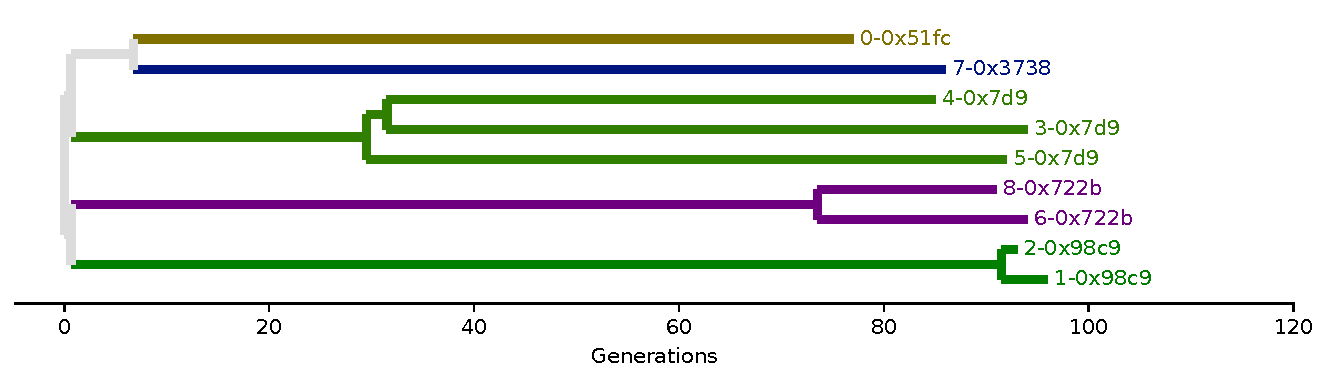
\includegraphics[width=\textwidth]{binder-wse-sketches/binder/teeplots/genome=hsurftiltedsticky_tagged+replicate=a2438095-6857-4a68-bd77-14065953b13c+viz=draw-biopython-tree+ext=}
    \caption{100 generations}
    \label{fig:tagged_other}
  \end{subfigure}
\end{figure*}
